\documentclass{article}
\usepackage[utf8]{inputenc}
\usepackage[french]{babel}
\usepackage{amsmath}
\usepackage{listings}
\usepackage{hyperref}
\usepackage{xcolor}
\usepackage{graphicx}
\usepackage[style=authoryear]{biblatex}
\usepackage{fancyhdr}
\usepackage{braket}
\usepackage{float}
\usepackage{color}

\definecolor{codegreen}{rgb}{0,0.6,0}
\definecolor{codegray}{rgb}{0.5,0.5,0.5}
\definecolor{codepurple}{rgb}{0.58,0,0.82}
\definecolor{backcolour}{rgb}{0.95,0.95,0.92}

\lstdefinestyle{mystyle}{
  backgroundcolor=\color{backcolour},   
  commentstyle=\color{codegreen},
  keywordstyle=\color{magenta},
  numberstyle=\tiny\color{codegray},
  stringstyle=\color{codepurple},
  basicstyle=\ttfamily\footnotesize,
  breakatwhitespace=false,         
  breaklines=true,                 
  captionpos=b,                    
  keepspaces=true,                 
  numbers=left,                    
  numbersep=5pt,                  
  showspaces=false,                
  showstringspaces=false,
  showtabs=false,                  
  tabsize=2
}

\pagestyle{fancy}

\fancyhf{}
\fancyhead[L]{Rapport de séminaire : L'algorithme quantique}
\fancyhead[R]{RAETH et SANNA, L3STI}
\fancyfoot[C]{Page n°\thepage}

\addbibresource{ref.bib}

\title{Rapport de séminaire :\\L'algorithme quantique}
\author{RAETH Léandre, SANNA Thomas\\L3 Sciences et Technologie  P. Informatique}
\date{\today}

\begin{document}

\maketitle

\tableofcontents

\break\section{Introduction}
\subsection{Présentation du sujet}
\subsection{Exemple introductif}

\break\section{Informatique classique vs. Informatique quantique}
\subsection{Bits classiques}
\subsection{Qubits quantiques}

\break\section{Propriétés fondamentales de l'informatique quantique}
\subsection{Superposition}
\subsection{Intrication}
\subsection{Interférence}

\break\section{Génération de Nombre aléatoire}
\subsection{Problématique}

Lors de la génération d'un nombre aléatoire en informatique traditionnelle, par exemple, en Python avec le module `random()`, le nombre généré est en réalité dit pseudo-aléatoire car l'algorithme de Mersenne Twister repose sur une graine pour initialiser le générateur de nombres aléatoires. Cette graine permet de prédire le prochain nombre pseudo-aléatoire, ce qui constitue un problème important pour de nombreux projets confidentiels, y compris la cryptographie.

Pour les projets impliquant une confidentialité sévère, comme la cryptographie, l'un des plus grands problèmes avec la génération de nombres pseudo-aléatoires est la capacité à produire des nombres élevés qui sont extrêmement difficiles à prédire. Par exemple, lors de la génération du sel du mot de passe afin de le hacher, un générateur de nombres aléatoires est utilisé. Si ce générateur est prévisible, un hacker compétent trouverait facilement le mot de passe en un rien de temps.

C'est pourquoi il est important de s'assurer que la graine choisie permettra un certain degré d'imprévisibilité.

En revanche, en informatique quantique, 
la génération de nombres aléatoires peut être véritablement aléatoire grâce aux propriétés 
quantiques expliquées il y a peu de temps. En effet, en utilisant un ordinateur 
quantique, on peut mesurer l'état d'un qubit en superposition pour obtenir un résultat aléatoire \b{non-déterministe} !

\subsection{Fonctionnement}

Pour comprendre comment fonctionne la génération de nombres aléatoires en informatique quantique, il faut se pencher sur les propriétés des qubits. Un qubit, comme on l'a vu plus tôt, peut être dans un état de superposition, ce qui signifie qu'il peut représenter simultanément les états 0 et 1. Lorsqu'on mesure un qubit en superposition, le résultat de la mesure est complètement aléatoire entre 0 et 1.

\begin{itemize}
  \item \textbf{Préparation du qubit} : On commence par préparer un qubit dans un état de superposition. Cela peut être réalisé en appliquant une porte Hadamard (H) à un qubit initialement dans l'état $\ket{0}$. La porte Hadamard transforme l'état $\ket{0}$ en une superposition égale des états $\ket{0}$ et $\ket{1}$ :
  \[
  H\ket{0} = \frac{1}{\sqrt{2}}(\ket{0} + \ket{1})
  \]
  La porte d'Hadamard est extrêmement utilisée en informatique quantique Ces superpositions ne sont pas des simulations de probabilités, mais des états réels qui peuvent être mesurés.
  \item \textbf{Mesure du qubit} : Une fois le qubit en superposition, on procède à sa mesure. La mesure d'un qubit en superposition donne un résultat aléatoire, soit 0 soit 1, avec une probabilité de 50\% pour chaque état. Ce processus est intrinsèquement aléatoire et ne peut pas être prédit, même si l'on connaît l'état initial du qubit.
  \item \textbf{Génération de séquences aléatoires} : En répétant ce processus de préparation et de mesure de qubits en superposition \texttt{n} fois, on peut générer des séquences de bits aléatoires. 
\end{itemize}

Ainsi, la génération de nombres aléatoires en informatique quantique repose sur les principes
fondamentaux de la mécanique quantique, offrant une source de véritable aléa, contrairement
aux méthodes pseudo-aléatoires utilisées en informatique classique. Nous pourrons trouver le code
de l'algorithme de génération de nombres aléatoires en informatique quantique dans la section suivante.


\subsection{Comparaison des méthodes}

\begin{table}[H]
  \centering
  \begin{tabular}{|c|c|}
    \hline
    \textbf{Informatique classique} & \textbf{Informatique quantique} \\
    \hline
    Pseudo-aléatoire & Non déterministe \\
    \hline
    Prédictible & Imprévisible \\
    \hline
    Basé sur des algorithmes & Basé sur des propriétés quantiques \\
    \hline
    Temps de calcul rapide & Temps de calcul plus lent \\
    \hline
  \end{tabular}
  \caption{Comparaison de la génération de nombres aléatoires en informatique classique et quantique}
\end{table}

\section{Expérimentation : coder un algorithme quantique}

\subsection{Introduction}

Il existe deux manières de coder un algorithme quantique : en utilisant un simulateur quantique
ou un véritable ordinateur quantique. Pour coder sur un vrai ordinateur quantique, il est possible
d'utiliser des services cloud comme IBM Quantum Experience, qui permettent d'accéder à des
ordinateurs quantiques en ligne. \cite{wikipediaQuantumPlatform}

Cependant, pour des raisons de simplicité, nous allons utiliser un simulateur quantique, qui
permet de simuler un ordinateur quantique sur un ordinateur classique. Pour cela, nous allons
utiliser le langage de programmation Qiskit.

En effet, Qiskit est un framework open-source développé par IBM en 2017 pour la programmation
d'algorithme quantique en Python \cite{wikipediaQiskitWikipedia}. Qiskit permettra d'utiliser cette fameuse 
porte Hadamard pour préparer un qubit dans un état de superposition.

\subsubsection{Les schémas de circuits quantiques}

Un circuit quantique est une représentation graphique d'un algorithme quantique. Il est composé
de qubits, de portes quantiques et de mesures. Les portes quantiques sont des opérations
unitaires qui agissent sur un ou plusieurs qubits. Les mesures permettent de lire l'état d'un qubit.

\textbf{Porte Hadamard} :
La porte de Hadamard, on l'a vu plus tôt, est une porte quantique qui permet de mettre un qubit
dans un état de superposition. Elle est représentée par la lettre H dans un schéma de circuit
quantique. Elle prend un qubit initialement dans l'état $\ket{0}$ (ou $\ket{1}$, peu importe, cela n'affectera pas la porte) et le transforme, à la sortie, en une superposition
équilibrée des états $\ket{0}$ et $\ket{1}$.

\begin{figure}[H]
  \centering
  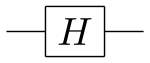
\includegraphics[width=0.3\textwidth]{img/hadamard.png}
  \caption{Schéma de circuit quantique pour la porte Hadamard (\cite{wikipediaPorteQuantique})}
\end{figure}

\textbf{Mesure} :
La mesure d'un qubit permet de lire son état. Elle est représentée par un symbole de balance dans
un schéma de circuit quantique. La mesure d'un qubit en superposition donne un résultat aléatoire
entre 0 et 1, avec une probabilité de 50\% pour chaque état. Elle prend dont un qubit en entrée et
renvoie un bit classique (0 ou 1) en sortie.

\textit{\textbf{Information :} Les deux lignes horizontales représentent un bit classique, tandis qu'une seule ligne représente un qubit.}

\begin{figure}[H]
  \centering
  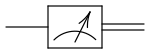
\includegraphics[width=0.3\textwidth]{img/mesure.png}
  \caption{Schéma de circuit quantique pour la mesure d'un qubit (\cite{wikipediaPorteQuantique})}
\end{figure}

\textbf{Circuit d'un algorithme de nombre aléatoire} :
Ce circuit quantique décris l'algorithme de génération de nombres aléatoires en informatique quantique. 

On travaille ici avec qu'un seul qubit \texttt{q} initialisé à l'état $\ket{0}$ ou $\ket{1}$ (conventionnellement, on choisit $\ket{0}$).
On applique ensuite une porte Hadamard à ce qubit pour le mettre dans un état de superposition. 
Enfin, on mesure le qubit pour obtenir un résultat aléatoire entre 0 et 1. 

Cette mesure est sortie dans la partie \texttt{c} du circuit (\texttt{c} signifie \textit{classique}).
Cette partie renvoie un bit classique, qui est le résultat de la mesure du qubit. En effet,
le \texttt{1} à droite de \texttt{c} signifie le nombre de bits classiques en sortie. Le \texttt{0}
à côté de la sortie de la mesure, signifie que le bit mesuré est à l'index numéro 0.


\begin{figure}[H]
  \centering
  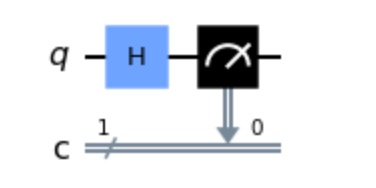
\includegraphics[width=0.5\textwidth]{img/portesLogiquesRandom.png}
  \caption{Portes logiques pour la génération d'un nombre aléatoire entre 0 et 1 (\cite{sapTrueRandomness})}
\end{figure}

\textbf{Circuit avec 8 qubits} :
Le problème avec le circuit précédent est qu'il ne génère qu'un seul bit aléatoire, ce qui veut dire que le nombre aléatoire généré est soit 0 soit 1. 
Pour générer un nombre aléatoire plus grand, il suffit de répéter le processus de préparation et de mesure de qubits en superposition plusieurs fois,
ou alors d'utiliser plusieurs qubits en superposition en même temps.

Ici, on obtient un circuit quantique pour la génération d'un nombre aléatoire avec 8 qubits.
En une seule exécution, ce circuit génère un nombre aléatoire entre 0 et 255 (car $2^8 = 256$).

\begin{figure}[H]
  \centering
  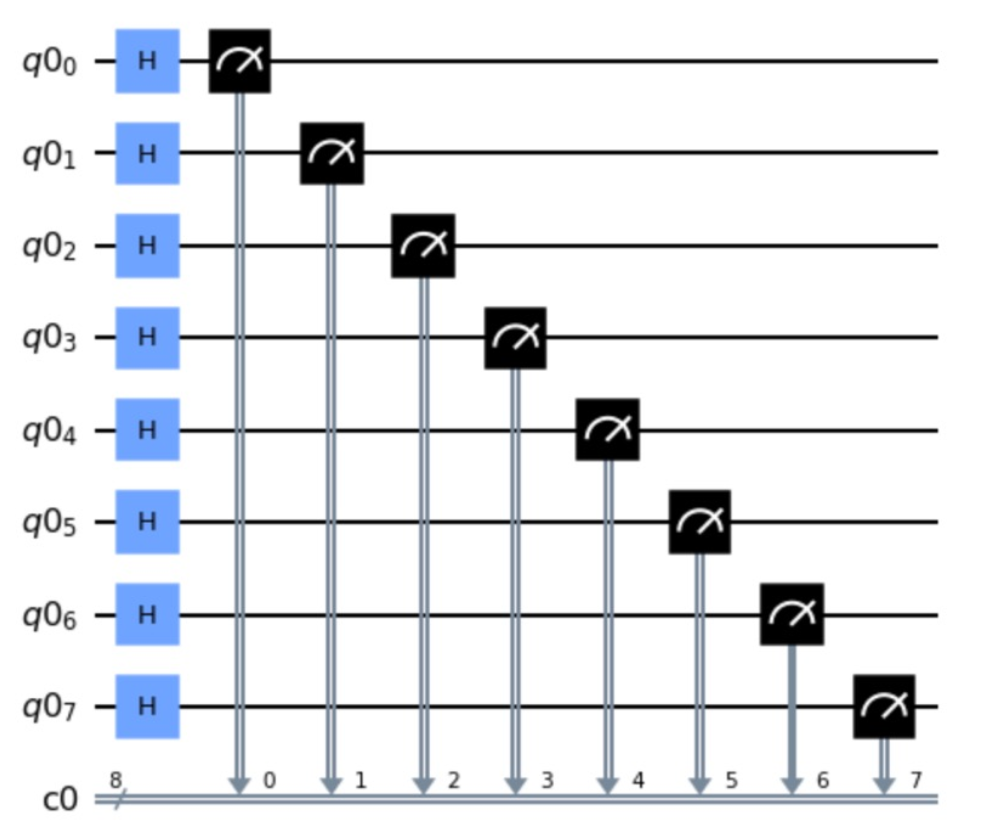
\includegraphics[width=0.7\textwidth]{img/portesLogiquesRandom8.png}
  \caption{Circuit quantique pour la génération d'un nombre aléatoire avec 8 qubits (\cite{sapTrueRandomness})}
\end{figure}

\subsection{Code de l'algorithme}

Dans cette partie, il est question de coder l'algorithme de génération de nombres aléatoires avec 8 qubits en informatique quantique en utilisant Qiskit.

\subsubsection{Prérequis}
Il est étonnament assez simple de coder un algorithme quantique en Python avec Qiskit. En voici les prérequis :

\begin{itemize}
  \item Installer Python : \texttt{https://www.python.org/downloads/}
  \item Installer Qiskit : \texttt{pip install qiskit}
  \item Installer Qiskit Aer : \texttt{pip install qiskit-aer} (\cite{qiskitGettingStarted})
\end{itemize}

Il est aussi préférable de coder sur Jupyter Notebook, qui permet d'exécuter du code Python en temps réel.

\subsubsection{Initialisation du circuit}

Le circuit quantique est initialisé avec 8 qubits en entrée et 8 bits classiques en sortie. On applique ensuite une porte Hadamard à chaque qubit pour les mettre dans un état de superposition, comme expliqué précédemment.
On mesure ensuite chaque qubit pour obtenir un résultat aléatoire entre 0 et 1, stocké dans leurs bits classiques respectifs. (Par exemple, le résultat du qubit 0 est stocké dans le bit classique 0, et ainsi de suite.)

\begin{lstlisting}[language=Python, style=mystyle, caption={Initialisation du circuit avec 8 qubits}]
  from qiskit import QuantumRegister, ClassicalRegister, QuantumCircuit
  from qiskit_aer import Aer
  
  q = QuantumRegister(8, 'q') # initialisation d'un registre quantique de 8 qubits
  c = ClassicalRegister(8, 'c') # initialisation d'un registre classique de 8 bits
  circuit = QuantumCircuit(q, c) # initialisation d'un circuit quantique avec les registres q et c
  
  circuit.h(q[0]) # porte de Hadamard sur le premier qubit
  circuit.h(q[1]) # porte de Hadamard sur le deuxieme qubit
  circuit.h(q[2]) # ...
  circuit.h(q[3])
  circuit.h(q[4])
  circuit.h(q[5])
  circuit.h(q[6])
  circuit.h(q[7])
  
  circuit.measure(q, c) # mesure de tous les qubits dans les bits classiques correspondants
\end{lstlisting}

\subsubsection{Exécution du circuit}

Pour exécuter le circuit, on utilise un simulateur quantique. Ici, on utilise le simulateur Aer de Qiskit, qui permet de simuler un ordinateur quantique sur un ordinateur classique.

À la fin de l'execution, on obtient en retour un dictionnaire contenant les résultats de la simulation, c'est-à-dire les nombres aléatoires générés.

\begin{lstlisting}[language=Python, style=mystyle, caption={Exécution du circuit}, label={lst:execution_circuit}]
  simulateur = Aer.get_backend('aer_simulator') # initialisation du simulateur Aer avec le backend aer_simulator
  circuitCompile = transpile(circuit, simulateur) # compilation du circuit pour le simulateur
  result = simulateur.run(circuitCompile, shots=1).result() # shot=1 veut dire qu'on execute le circuit une seule fois
  
  counts = result.get_counts(circuit)
  print("\nResultats de la mesure :", counts)  
\end{lstlisting}

\textit{\textbf{Note additionnelle} : On peut voir dans certains codes sur internet que le simulateur s'appelle \texttt{qasm\_simulator} au lieu de \texttt{aer\_simulator}. En effet, \texttt{qasm\_simulator} est une version nientôt obsolète du simulateur Aer. On conseille aujourd'hui d'utiliser \texttt{aer\_simulator} depuis peu. (\cite{stackexchangeWhatDifferences})}
\\ \\
En retour de cette exécution, on obtient un dictionnaire qui comporte le nombre binaire généré :
\begin{lstlisting}[style=mystyle, caption={Résultat de la mesure : \{'00001010': 1\}}]
  Resultats de la mesure : {'00001010': 1}
\end{lstlisting}
Ce dictionnaire contient le nombre binaire 8 bits généré, avec sa fréquence d'apparition. Il n'y a qu'une seule clé dans ce dictionnaire, qui est le nombre binaire généré, et la valeur associée est le nombre de fois que ce nombre a été généré (une seule fois car le circuit a été exécuté une fois, CF Listing \ref{lst:execution_circuit} \texttt{"shots=1"}).

Ici, le nombre généré est 00001010, qui correspond à 10 en décimal. On peut donc dire que le nombre aléatoire généré est 10.

\break\section{Limites et perspectives}
\subsection{Défis actuels}
\subsection{Futur de l'informatique quantique}

\break\section{Conclusion et Q\&A}
\subsection{Récapitulatif des points clés}
\subsection{Session de questions-réponses}

\break
\section{Bibliographie}
\printbibliography

\end{document}